\documentclass[a4paper,11pt]{article}

%%%%%%%%%%%%%%%%%%%%%
% pour écrire avec les accents directement dans le texte

\usepackage[numbers]{natbib} % Doit être chargé avant babel
\usepackage[frenchb,english]{babel}

 \usepackage[T1]{fontenc}
 \usepackage[utf8]{inputenc}
 \usepackage[colorlinks=false, urlcolor=black, breaklinks, pagebackref, citebordercolor={0 0 0}, filebordercolor={0 0 0}, linkbordercolor={0 0 0}, pagebordercolor={0 0 0}, runbordercolor={0 0 0}, urlbordercolor={0 0 0}, pdfborder={0 0 0}]{hyperref} 
%%%%%%%%%%%%%%%%%%%%% 

\usepackage{float}
\usepackage{amsmath}
\usepackage{amsfonts}
\usepackage{amssymb}
\usepackage{geometry}
\geometry{a4paper, margin=2.5cm, headheight=17pt}
\usepackage{graphicx}
\usepackage{hyperref}
\usepackage{icomma}
\usepackage{latexsym}
\usepackage{textcomp}
\usepackage[all]{xy}
\usepackage{cancel}
\usepackage{color}
\usepackage{dsfont}
\usepackage{subfig}
\usepackage{caption}
\usepackage{booktabs}
\usepackage{longtable}
\usepackage{dsfont}
\usepackage{extarrows}
\usepackage{shorttoc}
\usepackage{listings}
\usepackage{xcolor}
\usepackage{lmodern}
\usepackage{moreverb}
\usepackage{fancyhdr}

\lstset{
    basicstyle=\ttfamily\footnotesize,
    breaklines=true,
    frame=single,
    backgroundcolor=\color{gray!5}
}

\lstdefinelanguage{pseudo}{
    morekeywords={for,foreach,while,if,else,return},
    sensitive=false
}

   \newcommand{\bigO}[1]{\ensuremath{\mathop{}\mathopen{}O\mathopen{}\left(#1\right)}}
   \newcommand{\smallO}[1]{\ensuremath{\mathop{}\mathopen{}o\mathopen{}\left(#1\right)}}

\captionsetup{font=footnotesize}
\emergencystretch=1em

\setcounter{tocdepth}{3}

\makeatletter
\def\clap#1{\hbox to 0pt{\hss #1\hss}}%
\def\ligne#1{%
\hbox to \hsize{%
\vbox{\centering #1}}}%
\def\haut#1#2#3{%
\hbox to \hsize{%
\rlap{\vtop{\raggedright #1}}%
\hss
\clap{\vtop{\centering #2}}%
\hss
\llap{\vtop{\raggedleft #3}}}}%
\def\bas#1#2#3{%
\hbox to \hsize{%
\rlap{\vbox{\raggedright #1}}%
\hss
\clap{\vbox{\centering #2}}%
\hss
\llap{\vbox{\raggedleft #3}}}}%
\def\maketitle{%
\thispagestyle{empty}\vbox to \vsize{%
\haut{}{\@blurb}{}
\vfill
\vspace{0.5cm}
\hrule height 2pt
\vspace{0.2cm}
\par
\begin{center}
\fontseries{bx}
\huge \@title
\end{center}
\vspace{0.2cm}
\par
\hrule height 2pt
\par
\vspace{2cm}
\begin{center}
\Large
\textit{Auteurs:}
\end{center}
\begin{center}
\Large 
\@author
\par
\end{center}
\vspace{1cm}
\begin{center}
\Large
\textit{Responsables:}
\end{center}
\begin{center}
\Large 
Mathys E. Jam / Pablo Oliveira
\par
\end{center}
\vfill
\vfill
\bas{}{\begin{flushright}
\large
\@date
\end{flushright}}{}
}%
\cleardoublepage
}
\def\date#1{\def\@date{#1}}
\def\author#1{\def\@author{#1}}
\def\title#1{\def\@title{#1}}
\def\location#1{\def\@location{#1}}
\def\blurb#1{\def\@blurb{#1}}
\date{\today}
\author{}
\title{}
\location{}\blurb{%
\begin{center}

\includegraphics[width=20em]{Images/Logo_UVSQ.jpg}
\end{center}
}%
\makeatother
\title{Moteur d'Inférence de Réseaux de Neurones pour la Reconnaissance de Chiffres Manuscrits}
\author{Jianye SHI}
\date{\today}

% Configuration des en-têtes et pieds de page
\pagestyle{fancy}
\fancyhf{}
\fancyhead[L]{M1 CHPS -- UVSQ 25/26}
\fancyhead[R]{\leftmark}
\fancyfoot[C]{\thepage}
\renewcommand{\headrulewidth}{0.4pt}
\renewcommand{\footrulewidth}{0pt}
\setlength{\headheight}{17pt}

\begin{document}

% Page de titre sans en-tête ni pied de page
\maketitle

\renewcommand{\contentsname}{Sommaire}
\tableofcontents

\newpage

\section{Introduction}\label{sec:intro}

Ce projet s'inscrit dans le cadre de l'optimisation de performance et de l'implémentation de moteurs d'inférence pour réseaux de neurones. Il se compose de deux parties principales : l'optimisation d'un noyau SGEMM (Single-precision General Matrix Multiply) dans le Lab 6, puis l'utilisation de ce noyau optimisé pour implémenter un moteur d'inférence permettant la reconnaissance de chiffres manuscrits du dataset MNIST dans le Lab 7.

Le SGEMM est une opération fondamentale dans le calcul scientifique et l'apprentissage automatique, représentant souvent la majorité du temps de calcul dans les réseaux de neurones. L'optimisation de cette opération permet d'améliorer de manière notable les performances globales des applications. Dans ce travail, nous avons exploré plusieurs techniques d'optimisation : la réorganisation des boucles pour améliorer la localité mémoire ; le découpage en blocs pour maximiser l'utilisation du cache ; et la parallélisation avec OpenMP pour exploiter les architectures multi-cœurs.

Le moteur d'inférence développé dans le Lab 7 permet d'exécuter des modèles de réseaux de neurones au format ONNX, avec support pour quatre opérations de base : Flatten, Add, Relu et Gemm. L'objectif est de reconnaître des chiffres manuscrits avec une précision élevée tout en minimisant le temps d'exécution et la consommation énergétique.

\section{Environnement Expérimental}

Toutes les expériences ont été réalisées sur une machine avec les spécifications suivantes :

\subsection{Configuration Matérielle}

\begin{table}[H]
\centering
\caption{Configuration matérielle}
\label{tab:hardware}
\begin{tabular}{p{0.28\textwidth}p{0.62\textwidth}}
\toprule
\textbf{Composant} & \textbf{Caractéristiques} \\
\midrule
Processeur & \begin{tabular}[t]{@{}l@{}}
AMD Ryzen 9 8940HX with Radeon Graphics\\
Architecture : x86\_64\\
Cœurs / Threads : 16 physiques / 32 logiques (2 threads par cœur)\\
Fréquence : 421.8 MHz (min) à 5386 MHz (max)\\
Cache L1d : 512 KiB (16 instances)\\
Cache L1i : 512 KiB (16 instances)\\
Cache L2 : 16 MiB (16 instances)\\
Cache L3 : 64 MiB (2 instances)
\end{tabular} \\
Mémoire & 30 GiB de RAM système \\
Swap & 8.0 GiB \\
\bottomrule
\end{tabular}
\end{table}

Les expérimentations parallèles ainsi que les mesures d'énergie ont été réalisées sur cette même configuration matérielle.

\subsection{Configuration Logicielle}

\begin{table}[H]
\centering
\caption{Configuration logicielle}
\label{tab:software}
\begin{tabular}{p{0.28\textwidth}p{0.62\textwidth}}
\toprule
\textbf{Composant} & \textbf{Version / Détails} \\
\midrule
Système d'exploitation & Fedora Linux 42 (Workstation Edition) \\
Compilateur C/C++ & GCC 15.2.1 20250808 (Red Hat 15.2.1-1) \\
Python & Version 3.13.7 \\
CMake & Version 3.31.6 \\
Shell & zsh \\
IDE & Visual Studio Code on Linux \\
\bottomrule
\end{tabular}
\end{table}

Les mesures de performance ont été réalisées à l'aide de \texttt{perf stat} avec les événements RAPL (\texttt{power/energy-pkg/} et \texttt{power\_core/energy-core/}) pour quantifier la consommation énergétique. Les optimisations de compilation ont été testées avec les flags \texttt{-O3 -march=native} pour activer l'auto-vectorisation et les optimisations spécifiques à l'architecture.

\subsection{Protocole de mesure}\label{subsec:protocol}

Afin de limiter la variabilité des résultats, les campagnes de mesure suivent un protocole systématique de verrouillage de fréquence et d'affinité CPU. Les huit premiers cœurs physiques sont forcés à 4.0~GHz à l'aide de \texttt{cpupower}, puis les exécutions \texttt{perf stat} sont liées explicitement à ce jeu de cœurs via \texttt{taskset}. Le script type est le suivant :
Le détail des commandes (verrouillage de fréquence, événements suivi par \texttt{perf stat}, étapes de remise à l'état initial) est présenté en annexe~\ref{app:protocol}. Ce protocole constitue l'adaptation AMD des commandes recommandées pour les processeurs Intel dans le Lab~6, lesquelles préconisent un verrouillage similaire sur quatre cœurs logiques avec des bornes de fréquence adaptées au turbo (par exemple \texttt{cpupower frequency-set -g performance -u 5000MHz -d 5000MHz}). Les deux approches ne diffèrent donc que par les limites matérielles et la taille du groupe de cœurs réservés à l'expérience. Les scripts d'analyse acceptent les variables \texttt{LOCK\_FREQ} et \texttt{CPU\_SET} afin de rejouer automatiquement ces réglages.

\section{Implémentation et amélioration du SGEMM}\label{sec:sgemm}

\subsection{SGEMM naïf et analyse de performance initiale}\label{subsec:sgemm-naif}

L'opération SGEMM calcule $\text{RES} = A \times B + C$, où $A$ est une matrice $M \times K$, $B$ est une matrice $K \times N$, et $C$ et $\text{RES}$ sont des matrices $M \times N$. La version de base suit simplement trois boucles imbriquées :

\begin{lstlisting}[language=pseudo]
for each row i of A:
  for each column j of B:
    sum = dot(A[i, :], B[:, j])
    RES[i, j] = sum + C[i, j]
\end{lstlisting}

Cette implémentation naïve présente un problème de performance. Dans la boucle interne sur $k$, l'accès $B[k * N + j]$ parcourt $B$ avec un saut de $N$ éléments, traversant ainsi la matrice par colonnes (stride $N$) et générant de nombreux défauts de cache sur une organisation row-major.

Pour caractériser ce comportement, nous avons exécuté \texttt{sgemm naive} avec $N=K=512$ et $M$ croissant, en verrouillant la fréquence des cœurs selon le protocole décrit ci-dessus (Section~\ref{subsec:protocol}). La figure~\ref{fig:sizes} met en évidence une croissance quasi linéaire du temps d'exécution et de l'énergie consommée, ce qui est cohérent avec la complexité $O(MNK)$ lorsque deux dimensions sont fixées.

\begin{figure}[H]
\centering
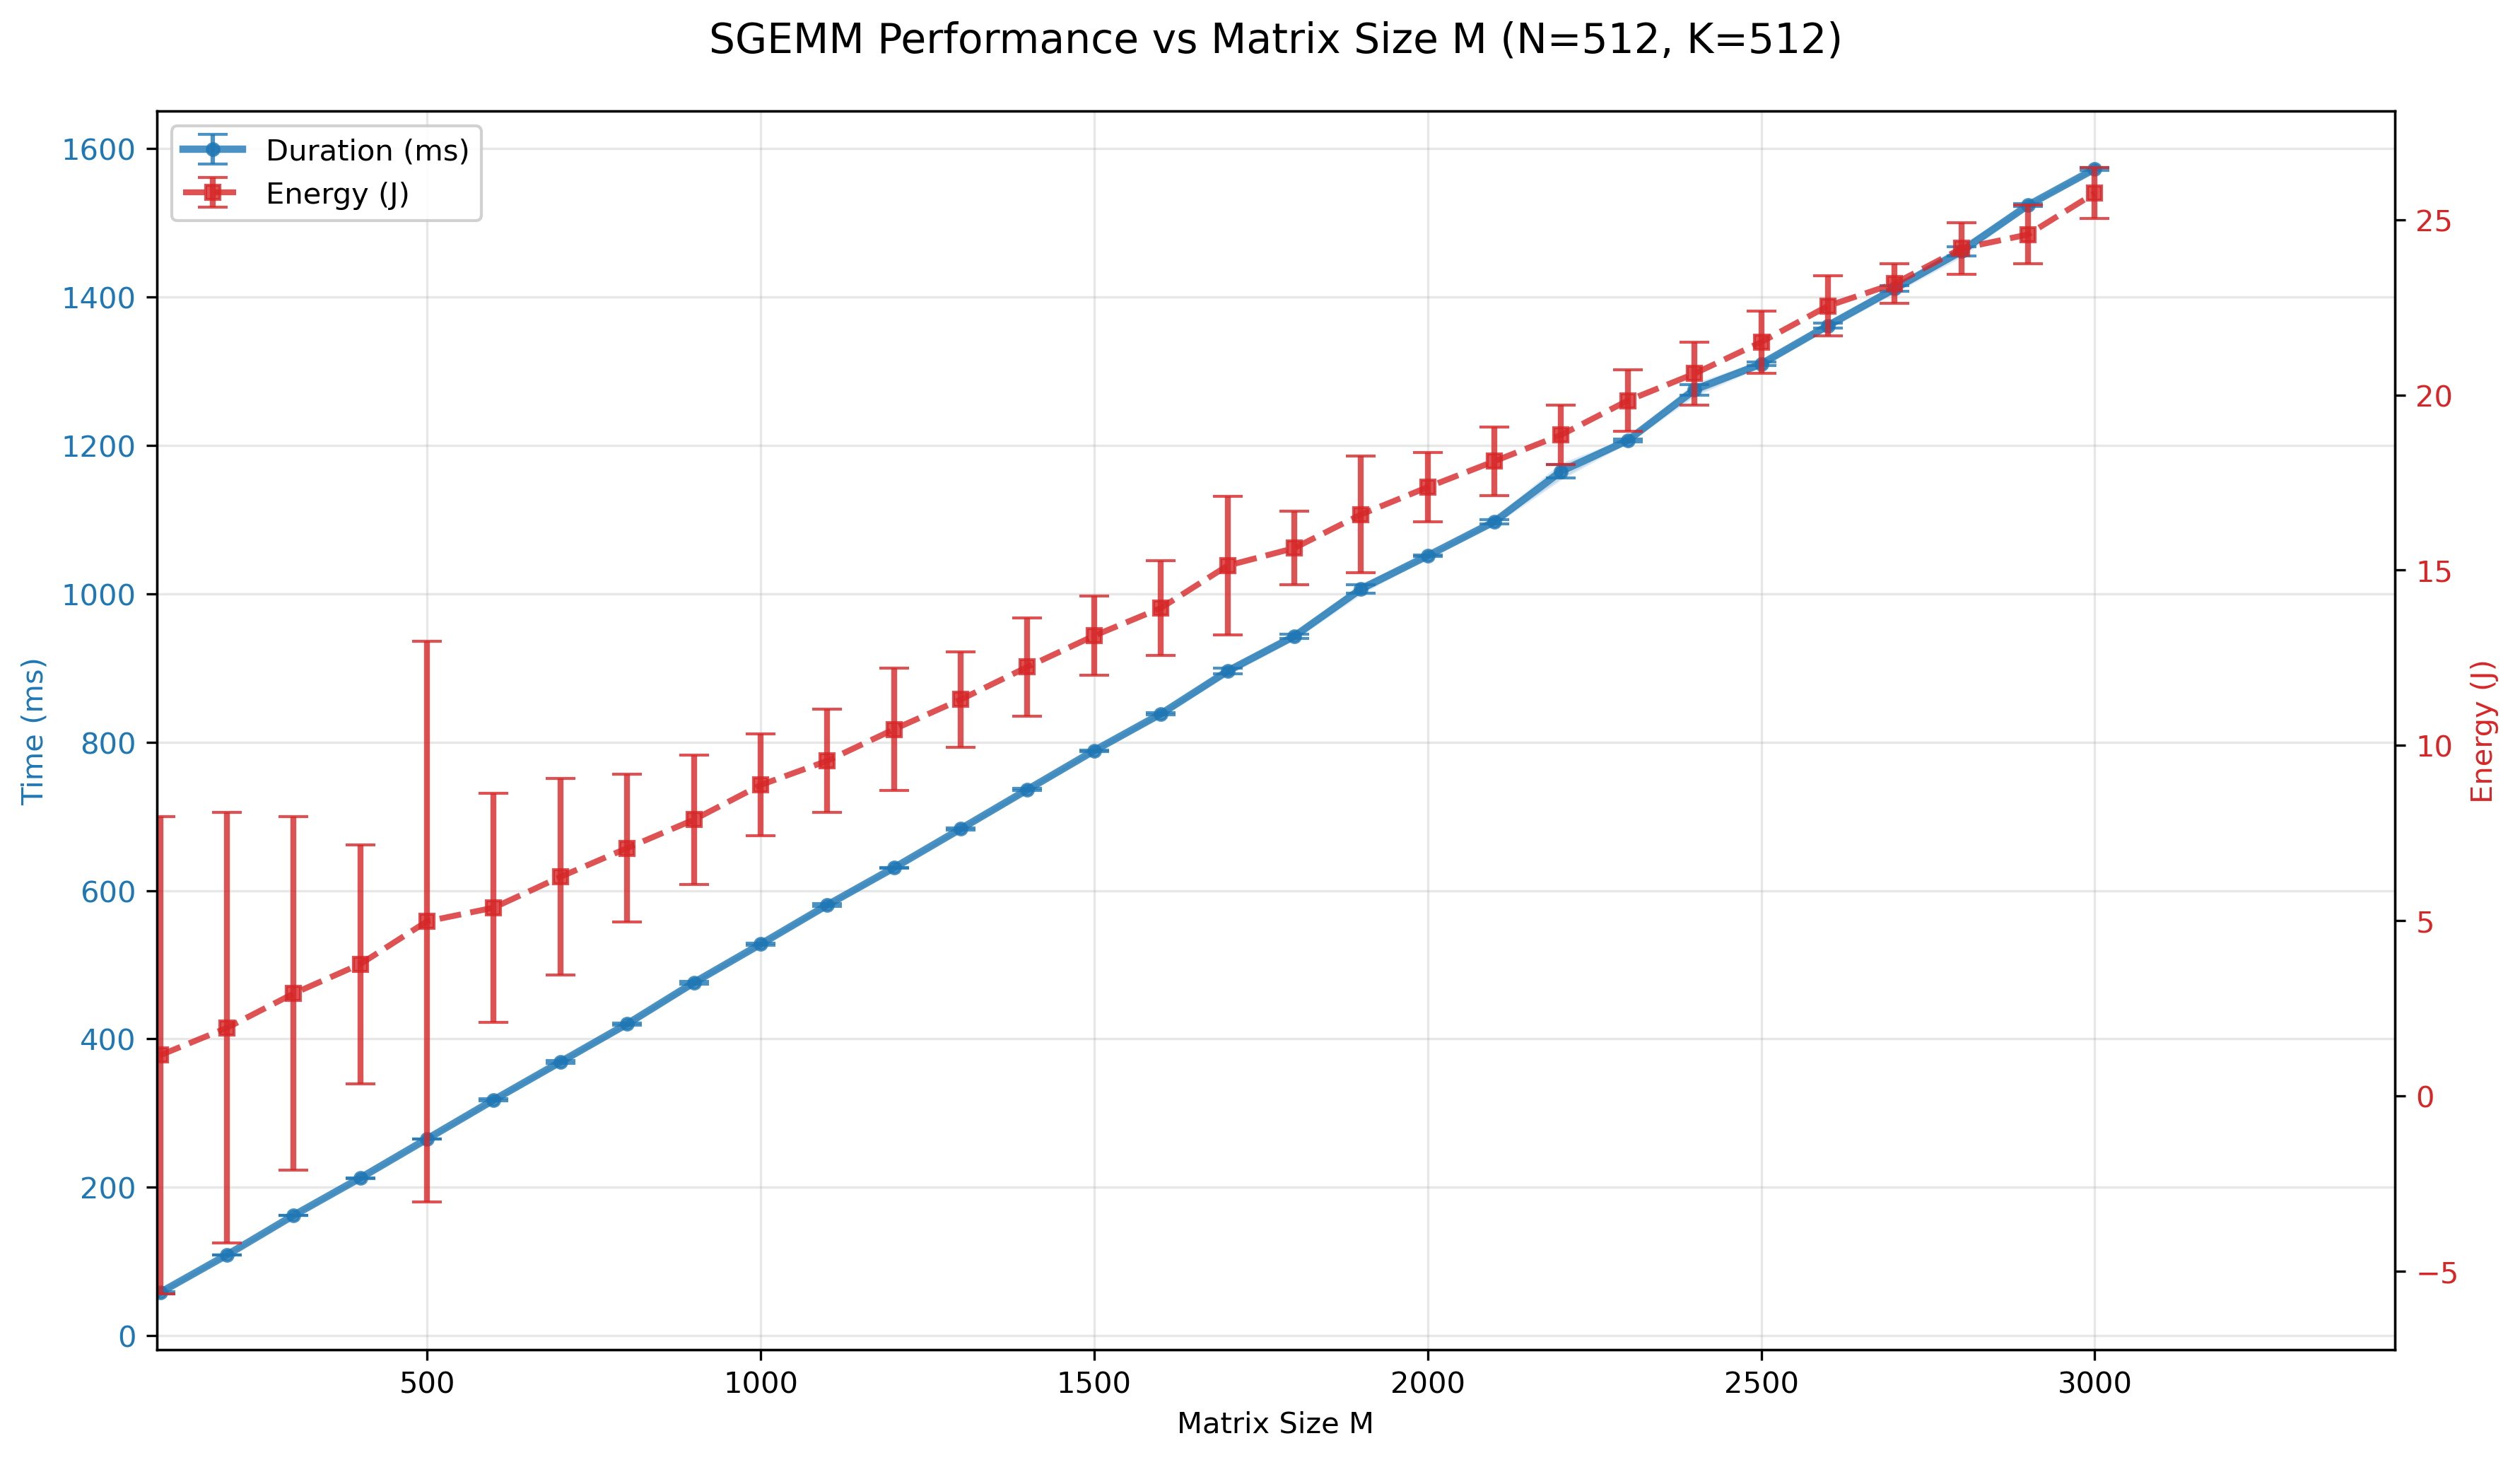
\includegraphics[width=0.8\textwidth]{Images/performance_naive.png}
\caption{Impact de la taille de matrice sur les performances (version naïve)}
\label{fig:sizes}
\end{figure}

Les barres d'erreur de l'énergie diminuent lorsque la taille de la matrice augmente, car les exécutions plus longues rendent la mesure RAPL plus stable et moins sensible aux variations instantanées de la puissance CPU.

Ces résultats illustrent la tendance de la version naïve ; nous l'utiliserons donc comme point de départ pour les optimisations qui suivent.

\subsection{Optimisations ikj, blockées et OpenMP}\label{subsec:sgemm-optim}

Les optimisations présentées ci-dessous visent à rapprocher le noyau SGEMM de l'idéal mémoire du processeur : la réorganisation ikj améliore la localité en parcourant séquentiellement les lignes de $B$ pour limiter les défauts de cache ; le découpage en blocs confine les données actives dans les niveaux rapides de la hiérarchie ; la parallélisation OpenMP étale enfin la charge restante sur plusieurs cœurs pour masquer les latences.

\paragraph{Réorganisation ikj.} Nous réorganisons les boucles dans l'ordre $(i, k, j)$ de façon à parcourir $A$ et $B$ ligne par ligne. Concrètement, on initialise $\text{RES}$ avec $C$, puis pour chaque couple $(i, k)$ on additionne la ligne $B[k, :]$ pondérée par $A[i, k]$. Cette structure évite les accès en colonne dans $B$ et réduit drastiquement les défauts de cache, d'où le nom de variante \texttt{sgemm\_ikj}. L'usage systématique des pointeurs \texttt{restrict} indique au compilateur l'absence d'alias, ce qui favorise l'auto-vectorisation.

\paragraph{Découpage en blocs.} La variante \texttt{sgemm\_blocked} découpe les trois boucles selon un pas de 128, de sorte que chaque itération travaille sur un sous-ensemble borné des matrices $A$, $B$ et $\text{RES}$. Les données actives demeurant confinées à ces sous-régions, les accès traversent moins de lignes de cache ; la hiérarchie matérielle assure alors une meilleure réutilisation des blocs en L1/L2, ce qui améliore la localité et réduit le taux de défauts.

\paragraph{Parallélisation OpenMP.} À partir du noyau \texttt{ikj}, nous parallélisons la boucle externe sur les blocs (ou lignes) de $\text{RES}$ au moyen d'OpenMP. Le planificateur \texttt{schedule(static)} assure que chaque thread reçoit le même nombre de blocs, ce qui offre un partage de charge efficace pour des matrices régulières.

\paragraph{Optimisations de compilation.} Enfin, les options \texttt{-O3 -march=native} activent l'auto-vectorisation et l'utilisation des instructions SIMD spécifiques à l'architecture (AVX2/AVX-512 sur notre machine), complétant les gains obtenus par les transformations algorithmiques précédentes.

\subsection{Analyse de performance après optimisation}\label{subsec:sgemm-perf}

Les mesures de performance ont été effectuées à l'aide de \texttt{perf stat} afin d'observer l'impact des optimisations sur le temps, l'énergie et les compteurs matériels. Nous utilisons la version monothread d'OpenBLAS comme cible idéale à atteindre sur CPU. L'ensemble des résultats présentés ci-dessous suit le protocole expérimental décrit en Section~\ref{subsec:protocol}.

La mesure de référence est résumée dans le tableau~\ref{tab:baseline} : elle porte sur 20 répétitions de \texttt{sgemm naive 512 512 512} avec les mêmes réglages d'affinité et de fréquence.

\begin{table}[H]
\centering
\caption{Mesure de référence pour \texttt{sgemm naive 512 512 512}}
\label{tab:baseline}
\begin{tabular}{lccc}
\toprule
Test & Répétitions & Temps moyen (s) & Énergie pkg (J) \\
\midrule
\texttt{sgemm naive 512 512 512} & 20 & 0.27599 & 10.26 \\
\bottomrule
\end{tabular}
\end{table}

Deux scripts automatisent ensuite le balayage de $M$ (avec $N=K=512$) :
\begin{itemize}
    \item \texttt{performance/compare-sizes.sh}, qui produit le CSV \texttt{performance/sgemm\_sizes\_com- parison.csv} ;
    \item \texttt{performance/plot-sizes.py}, qui transforme ce CSV en figure~\ref{fig:sizes}.
\end{itemize}
Le script \texttt{performance/compare-optimizations.sh} évalue \texttt{naive}, \texttt{ikj}, \texttt{blocked}, \texttt{omp} (1--16 threads) et \texttt{blas} pour $M \in \{512,1024,2048,4096\}$. Les cycles, instructions et mesures RAPL sont stockés dans un CSV long, puis \texttt{performance/plot-optimizations.py} synthétise directement les distributions de temps et d'énergie (notamment pour $M=512$ et $M=4096$) qui alimentent la figure~\ref{fig:comparison}.

La figure~\ref{fig:comparison} illustre la comparaison détaillée des différentes versions optimisées pour $M=512$ et $M=4096$, mettant en parallèle les effets sur le temps et l'énergie.

\begin{figure}[H]
\centering

\includegraphics[width=0.9\textwidth]{Images/performance_optimizations_dual_small.png}\\[0.5em]

\includegraphics[width=0.9\textwidth]{Images/performance_optimizations_dual_large.png}
\caption{Comparaison des performances et de la consommation d'énergie des différentes implémentations de SGEMM pour deux tailles de matrice}
\label{fig:comparison}
\end{figure}

\paragraph{Observations clés.} Plusieurs enseignements ressortent de ces campagnes :

\begin{itemize}
\item \textbf{Localité mémoire} : la variante ikj apporte le gain le plus significatif en supprimant les accès discontinus.
\item \textbf{Parallélisation} : l'ajout de threads OpenMP réduit fortement le temps d'exécution jusqu'à 8 threads, puis le gain se tasse ; pour $M=4096$, passer de 8 à 16 threads divise encore presque par deux le temps mais avec un rendement décroissant.
\item \textbf{Consommation énergétique} : l'énergie chute nettement entre 1 et 8 threads, puis se stabilise ; les configurations 8T et 16T affichent des consommations proches alors que la seconde reste plus rapide.
\end{itemize}


\paragraph{Comparaison des versions optimisées.}

Le tableau~\ref{tab:optimizations} présente les résultats de performance pour différentes implémentations sur une matrice $512 \times 512 \times 512$. La version \texttt{ikj} apporte une accélération d'environ 14x par rapport à la version naïve, principalement grâce à l'amélioration de la localité mémoire. La version blocked offre des performances similaires, avec une légère amélioration pour les grandes matrices. La version OpenMP atteint environ 24x à 8 threads et 25x à 16 threads, les gains devenant marginaux au-delà.

\begin{table}[H]
\centering
\caption{Comparaison des performances SGEMM (M=512, N=512, K=512)}
\label{tab:optimizations}
\begin{tabular}{lrrr}
\toprule
Version & Temps (ms) & Énergie (J) & Accélération \\
\midrule
naive & 273.6 & 11.25 & 1.0x \\
ikj & 19.6 & 0.99 & 14.0x \\
blocked & 19.4 & 1.04 & 14.1x \\
omp (8 threads) & 11.3 & 0.51 & 24.2x \\
omp (16 threads) & 10.7 & 0.51 & 25.5x \\
blas & 12.8 & 0.53 & 21.4x \\
\bottomrule
\end{tabular}
\end{table}

Des campagnes complémentaires ont été menées pour caractériser l'impact de la vectorisation, du comportement des caches et de l'affinité OpenMP.

\subsection{Impact de la vectorisation}\label{subsec:vectorization}
Le binaire \texttt{build-o3} est compilé avec \texttt{-O3 -march=native -fopt-info-vec-optimized}. Le journal \texttt{performance/vectorization\_build.log} atteste que les noyaux \texttt{naive}, \texttt{ikj}, \texttt{blocked} et \texttt{omp} disposent de boucles vectorisées (largeurs 64B/32B/16B). Les campagnes de mesure \texttt{perf}, comparant \texttt{build/sgemm} et \texttt{build-o3/sgemm} donnent les tendances résumées dans le tableau~\ref{tab:vectorization}. Les gains sont les plus marqués en mono-thread (jusqu'à $1.30\times$ sur \texttt{naive}), puis décroissent à mesure que la mémoire devient le facteur limitant.

\begin{table}[H]
\centering
\caption{Effet de la vectorisation (\texttt{performance/sgemm\_perf\_default.csv} vs \texttt{performance/sgemm\_perf\_vectorized.csv})}
\label{tab:vectorization}
\begin{tabular}{lcc}
\toprule
Implémentation & Accélération moyenne & Variation d'énergie \\
\midrule
\texttt{naive} (1 thread) & $\approx 1.30\times$ & $-20\%$ à $-35\%$ \\
\texttt{ikj} (1 thread) & $1.28$--$1.40\times$ & $-15\%$ à $-25\%$ \\
\texttt{blocked} / \texttt{blas} & $1.05$--$1.18\times$ & $-10\%$ à $-20\%$ \\
\texttt{omp} (2--4 threads) & $1.20$--$1.45\times$ & $-10\%$ à $-18\%$ \\
\texttt{omp} (8+ threads) & $\leq 1.10\times$ & baisse modérée, bénéfice limité par le débit mémoire \\
\bottomrule
\end{tabular}
\end{table}

Au-delà de huit threads, l'accès mémoire devient prépondérant : la vectorisation conserve un léger avantage énergétique mais ne change plus significativement le temps d'exécution.

\subsection{Analyse des événements de cache}\label{subsec:cache-events}
Les mesures \texttt{perf stat} sur $M=1280$, $N=K=512$ révèlent l'effet cumulé du réordonnancement et du blocage de boucle (tableau~\ref{tab:cache}). Les colonnes listent les compteurs AMD L3 et les défauts L1.

\begin{table}[H]
\centering
\caption{Comptage des événements de cache (extrait \texttt{performance/sgemm\_cache})}
\label{tab:cache}
\begin{tabular}{lrrrrr}
\toprule
Version & L3 cohérents & L3 hits & L3 miss & L1 miss & Temps (s) \\
\midrule
\texttt{naive} & $2.79\times 10^{7}$ & $2.64\times 10^{7}$ & $1.58\times 10^{6}$ & $3.76\times 10^{8}$ & 0.6744 \\
\texttt{ikj} & $1.35\times 10^{7}$ & $1.21\times 10^{7}$ & $1.33\times 10^{6}$ & $2.73\times 10^{7}$ & 0.0431 \\
\texttt{blocked} & $4.28\times 10^{6}$ & $3.05\times 10^{6}$ & $1.22\times 10^{6}$ & $3.67\times 10^{7}$ & 0.0430 \\
\bottomrule
\end{tabular}
\end{table}

Le passage à \texttt{ikj} divise par deux les accès L3 cohérents et réduit d'un ordre de grandeur les défauts L1. La version \texttt{blocked} se concentre sur des sous-blocs: elle abaisse encore la pression sur le L3 tout en maintenant un temps similaire à \texttt{ikj}.

\subsection{Réglages d'affinité OpenMP}\label{subsec:omp-affinity}
Pour $M=2048$, $N=K=512$ et huit threads, \texttt{performance/experiment-omp-affinity.sh} compare plusieurs réglages d'affinité (tableau~\ref{tab:affinity}). Les mesures confirment que le placement homogène sur les cœurs physiques est préférable.

\begin{table}[H]
\centering
\caption{Impact des stratégies OpenMP (8 threads)}
\label{tab:affinity}
\begin{tabular}{lrr}
\toprule
Configuration & Temps (ms) & Énergie pkg (J) \\
\midrule
Défaut (auto) & 25.11 & 1.65 \\
OMP\_PLACES=cores, PROC\_BIND=close & 24.95 & 1.61 \\
OMP\_PLACES=cores, PROC\_BIND=spread & 25.02 & 1.64 \\
Empilement forcé (threads sur mêmes cœurs) & 42.00 & 2.24 \\
\bottomrule
\end{tabular}
\end{table}

Contraindre plusieurs threads sur un même cœur logique dégrade simultanément temps et énergie.

Ces optimisations constituent le socle logiciel sur lequel s'appuie le moteur d'inférence présenté dans la section~\ref{sec:engine}.

\vspace{2\baselineskip}

\section{Moteur d'Inférence de Réseaux de Neurones}\label{sec:engine}

Le moteur d'inférence résultant du Lab~7 exécute des modèles ONNX générés par PyTorch. Il réutilise le noyau SGEMM optimisé pour accélérer les couches \texttt{Gemm}, ce qui en fait l'élément central des performances de bout en bout.

\subsection{Architecture générale}

Pour clarifier la répartition des responsabilités logicielles, le tableau~\ref{tab:engine-files} résume les fichiers centraux du moteur et les points remarquables à retenir pour l'analyse de performance.

\begin{table}[H]
\centering
\caption{Synthèse des principaux fichiers du moteur d'inférence}
\label{tab:engine-files}
\begin{tabular}{|p{0.25\textwidth}|p{0.33\textwidth}|p{0.32\textwidth}|}
\hline
\textbf{Fichier} & \textbf{Rôle principal} & \textbf{Points notables} \\
\hline
\texttt{src/main.c} & Interface CLI et chargement du modèle & Options \texttt{--gemm}, \texttt{--profile}, gestion des chemins ONNX \\
\hline
\texttt{src/inference.c} & Orchestration des opérateurs & Implémentations de Flatten, Relu, Gemm et Add, sélection du backend SGEMM \\
\hline
\texttt{src/inference.h} & Structures de données partagées & Définit \texttt{matrix\_t}, signatures publiques de l'API inference \\
\hline
\texttt{src/parse\_model.c} & Chargement et description du graphe & Parcours des noeuds ONNX, création de \texttt{value\_map} \\
\hline
\texttt{external/sgemm/\newline sgemm.c} & Noyaux de multiplication optimisés & Variantes \texttt{naive}, \texttt{ikj}, \texttt{blocked} et \texttt{omp} avec \texttt{schedule(static)} \\
\hline
\end{tabular}
\end{table}

\paragraph{Représentation des données.} Les tenseurs sont encapsulés dans la structure \texttt{matrix\_t} (dimensions, indicateur \texttt{weights}, pointeur sur les données). Les poids sont chargés une seule fois depuis le fichier ONNX et conservés en mémoire row-major pour rester compatibles avec l'ensemble des backends SGEMM (\texttt{sgemm\_ikj}, \texttt{sgemm\_omp}, etc.).

\paragraph{Graphe de calcul.} Le modèle ONNX est traité comme un graphe acyclique dirigé : chaque nœud représente un opérateur et les arêtes matérialisent le flux de tenseurs. Le parseur (basé sur \texttt{onnx-ml.pb-c}) expose des fonctions de navigation permettant de récupérer les entrées, sorties et initialisateurs de chaque nœud.

\subsection{Opérateurs supportés}

\paragraph{Flatten.} Conversion d'un tenseur $(N, M)$ en vecteur colonne $(NM, 1)$ via une simple copie séquentielle.

\paragraph{Add.} Addition élément par élément de deux matrices de même forme, opération linéaire aisément vectorisable.

\paragraph{Relu.} Application de $\max(0, x)$ sur chaque valeur ; le compilateur vectorise cette boucle simple.

\paragraph{Gemm.} Calcul de $Y = W \times X + B$ en s'appuyant sur le backend SGEMM sélectionné à l'exécution. Nous utilisons \texttt{sgemm\_ikj} par défaut, \texttt{sgemm\_omp} pour les campagnes multi-thread, tandis que \texttt{sgemm\_blocked} et \texttt{sgemm\_blas} servent de points de comparaison. Cette intégration directe assure que les optimisations mémoire (ikj, blocage, parallélisation OpenMP) sont réutilisées dans le moteur.

\subsection{Planificateur d'exécution}

Le moteur maintient une table de correspondance (\texttt{value\_map}) associant chaque nom de tenseur à sa matrice courante.

\paragraph{Gestion mémoire.} Chaque entrée précise si le tenseur est possédé par le moteur (allocation interne) ou emprunté au graphe (poids). À la fin de l'exécution, les buffers temporaires sont libérés automatiquement, ce qui évite les fuites tout en réutilisant les poids.

\paragraph{Ordonnancement.} Les nœuds sont parcourus dans l'ordre topologique fourni par ONNX ; un nœud n'est évalué que lorsque l'ensemble de ses entrées figure dans \texttt{value\_map}. Cette stratégie simple suffit puisque les modèles étudiés ne contiennent pas de branchement conditionnel.

\subsection{Validation et tests}

\paragraph{Tests unitaires.} Chaque opérateur possède des tests basés sur Unity qui couvrent différentes dimensions et vérifient la précision numérique avec une marge d'erreur serrée.

\paragraph{Validation MNIST.} Nous avons exécuté 100 images (\texttt{image\_0.ubyte} à \texttt{image\_99.ubyte}) sur trois modèles ONNX de complexité croissante, en forçant toutes les passes à utiliser l'implémentation multi-thread \texttt{sgemm\_omp} (\texttt{OMP\_NUM\_THREADS}=16). Les résultats sont présentés dans le tableau~\ref{tab:mnist}.

\begin{table}[H]
\centering
\caption{Résultats de reconnaissance sur le dataset MNIST}
\label{tab:mnist}
\small
\begin{tabular}{lrrr}
\toprule
Modèle & Précision & Temps (ms) & Énergie pkg (J) \\
\midrule
mnist.onnx & 98\% & 72{,}8 & 0{,}41 \\
mnist2.onnx & 97\% & 70{,}0 & 0{,}33 \\
mnist\_big.onnx & 98\% & 103{,}9 & 1{,}48 \\
\bottomrule
\end{tabular}
\end{table}

Tous les modèles atteignent une précision supérieure à 97\%, démontrant la correctitude de l'implémentation. Le modèle \texttt{mnist\_big.onnx} reste le plus coûteux à cause de sa profondeur accrue. Les mesures RAPL activées pendant la campagne multi-thread indiquent une dépense moyenne par image comprise entre 0,33 et 1,48~J sur le package CPU.

\vspace{2\baselineskip}

\section{Analyse de performance du moteur}

\subsection{Les mesures de performance}
Les mesures rassemblées au tableau~\ref{tab:mnist} mettent en évidence le lien direct entre la taille du réseau et le temps d'inférence. En configuration \texttt{sgemm\_omp} (16 threads), le moteur traite une image MNIST en 72{,}8~ms pour \texttt{mnist.onnx} et 70{,}0~ms pour \texttt{mnist2.onnx}, tandis que le modèle plus profond \texttt{mnist\_big.onnx} requiert 103{,}9~ms. La consommation énergétique moyenne par image passe simultanément de 0{,}33~J à 1{,}48~J selon la complexité du modèle.

\subsection{CLI \texttt{--gemm} / \texttt{--profile} et mesure des opérateurs}
Le point d'entrée \texttt{main.c} accepte désormais l'option \texttt{--gemm=<backend>} qui sélectionne dynamiquement l'implémentation SGEMM à l'exécution (\texttt{ikj}, \texttt{blocked}, \texttt{omp}, etc.). L'appel est relayé à \texttt{inference\_set\_gemm\_backend()} avant le chargement du modèle, ce qui permet de comparer plusieurs variantes sans recompiler. 

L'option \texttt{--profile} instruit \texttt{src/inference.c} pour chronométrer chaque appel à \texttt{Flatten}, \texttt{Add}, \texttt{Relu} et \texttt{Gemm} avant d'émettre un bloc \texttt{PROFILE\_JSON}. Les campagnes automatisées activent les variables d'environnement \texttt{PROFILE\_INFERENCE=1}, \texttt{MEASURE\_ENERGY=1} et \texttt{REPEAT=1}, fixent \texttt{GEMM\_BACKEND=omp} avec \texttt{OMP\_NUM\_THREADS}=16 et laissent \texttt{CPU\_SET} non contraint. Les traces consolidées dans \texttt{performance/results.json} sont ensuite synthétisées par
\begin{center}
\texttt{performance/profile\_charts.py --input performance/results.json --output performance/charts}
\end{center}
pour produire les graphiques de la figure~\ref{fig:mnist-profiles}. Sur ce lot de mesures, \texttt{Gemm} concentre 83{,}8~\% du temps total pour \texttt{mnist} et 79{,}4~\% pour \texttt{mnist2}, mais seulement 32{,}1~\% pour \texttt{mnist\_big}. Le temps non attribué correspond aux copies de tenseurs, aux allocations intermédiaires et aux synchronisations OpenMP, tandis que \texttt{Relu} et \texttt{Add} restent chacun sous la barre du pourcent.

\begin{table}[H]
    \centering
    \caption{Profils temporels et nombre d'appels par opérateur GEMM pour les modèles \texttt{mnist}, \texttt{mnist2} et \texttt{mnist\_big}}
    \label{tab:mnist}
    \small
\begin{tabular}{lrrr}
\toprule
Modèle & Temps (ms) & Pourcentage du temps total & Nombre d'appels \\
\midrule
mnist.onnx & 389{,}67 & 83{,}8 & 700 \\
mnist2.onnx & 260{,}04 & 79{,}4 & 500 \\
mnist\_big.onnx & 363{,}41 & 32{,}1 & 700 \\
    \bottomrule
    \end{tabular}
    \end{table}

\begin{figure}[H]
\centering
\begin{minipage}{0.48\textwidth}
    \centering
    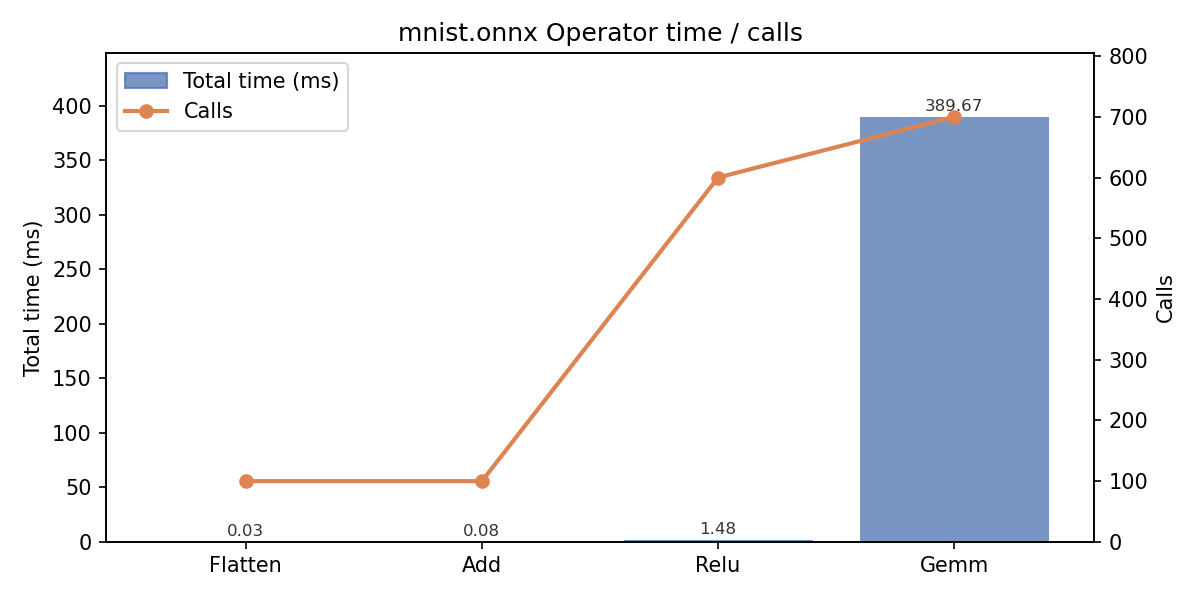
\includegraphics[width=\textwidth]{Images/profile_ops_time_calls_mnist_onnx.png}
\end{minipage}\hfill
\begin{minipage}{0.48\textwidth}
    \centering
    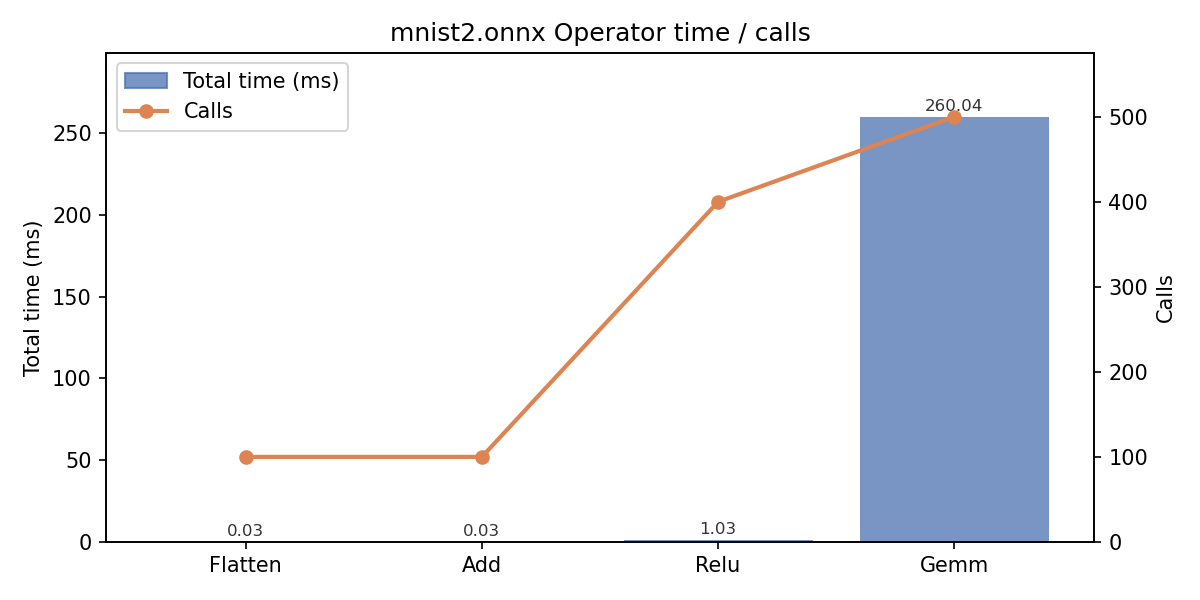
\includegraphics[width=\textwidth]{Images/profile_ops_time_calls_mnist2_onnx.png}
\end{minipage}

\vspace{0.6em}

\begin{minipage}{0.48\textwidth}
    \centering
    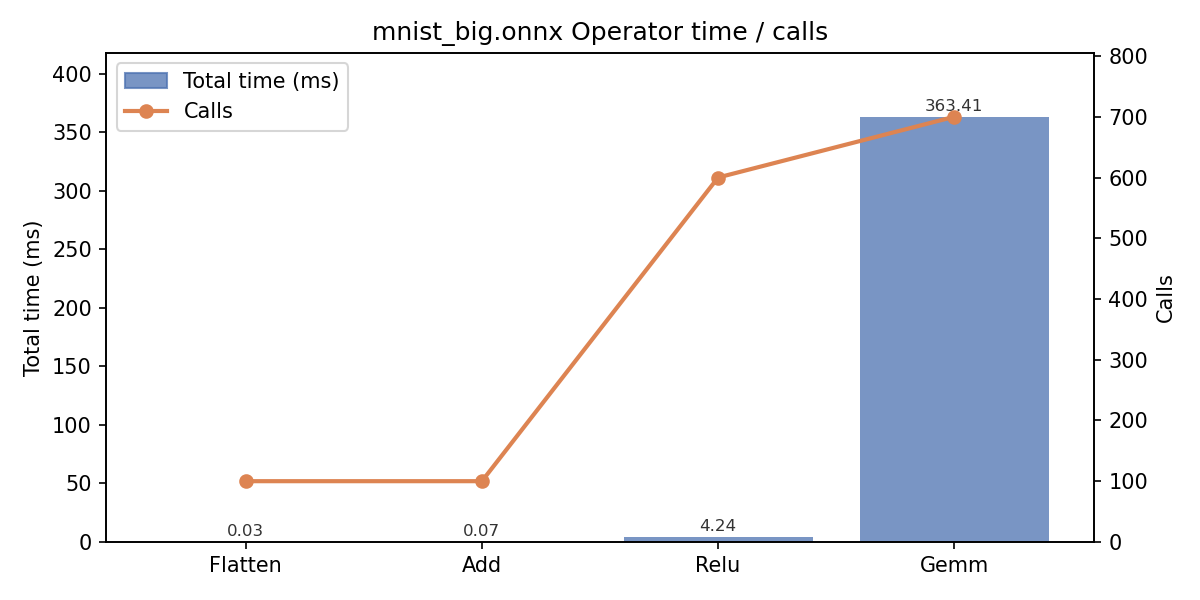
\includegraphics[width=\textwidth]{Images/profile_ops_time_calls_mnist_big_onnx.png}
\end{minipage}
\caption{Profils temporels et nombre d'appels par opérateur pour les modèles \texttt{mnist}, \texttt{mnist2} et \texttt{mnist\_big}}
\label{fig:mnist-profiles}
\end{figure}

\subsection{Impact des variantes SGEMM sur l'inférence (analyse qualitative)}
Les campagnes actuelles n'évaluent que l'implémentation multi-thread \texttt{sgemm\_omp}. Toutefois, les résultats du Lab~6 indiquent qu'une version naïve allongerait d'un facteur 24 le temps des couches Gemm, rendant l'inférence globale prohibitive. À l'inverse, des variantes mono-thread optimisées (\texttt{sgemm\_ikj}) ou vectorisées promettent encore des gains importants, notamment pour \texttt{mnist\_big.onnx}.

\vspace{2\baselineskip}

\section{Conclusion}\label{sec:conclusion}

Ce projet a permis de développer et d'optimiser un moteur d'inférence de réseaux de neurones pour la reconnaissance de chiffres manuscrits. Les principaux résultats sont :

\begin{itemize}
\item L'optimisation du noyau SGEMM a permis d'atteindre une accélération de 24x par rapport à l'implémentation naïve, principalement grâce à l'amélioration de la localité mémoire et la parallélisation.

\item Le moteur d'inférence atteint une précision de 97-98\% sur le dataset MNIST, démontrant la correctitude de l'implémentation.

\item Les mesures de performance indiquent des temps d'inférence compris entre 70 et 104 ms par image avec le backend \texttt{sgemm\_omp} (16 threads) dans les cores 0-7 et fréquence donnée par le CPU, pour une énergie moyenne par image allant de 0,33 à 1,48~J sur le package.

\item L'analyse révèle que les opérations Gemm restent prépondérantes sur \texttt{mnist} et \texttt{mnist2} (79--84~\% du temps total), mais ne représentent que 32~\% sur \texttt{mnist\_big}, le reste provenant des coûts de gestion multi-thread.
\end{itemize}

Les travaux futurs pourraient explorer l'optimisation SIMD explicite, la fusion d'opérateurs, et l'inférence par lots pour améliorer encore les performances et l'efficacité énergétique.

\appendix
\section{Scripts expérimentaux et protocoles}\label{sec:appendix-scripts}

\subsection{Protocole de mesure}\label{app:protocol}
\begin{lstlisting}[language=bash]
sudo cpupower frequency-set -g performance -u 4000MHz -d 4000MHz
# power/energy-pkg/ : total package energy
# power_core/energy-core/ : core execution energy
# USE_SUDO=1 : pour forcer l'usage de sudo dans les scripts
USE_SUDO=1 sudo taskset -c 0-7 perf stat -r 20 -a -C 0-7 \
    -e duration_time,power/energy-pkg/,power_core/energy-core/ \
    ./build/sgemm naive 512 512 512

sudo cpupower frequency-set -g powersave
sudo cpupower frequency-set -d 421MHz -u 5386MHz
\end{lstlisting}

\subsection{Balayage des tailles}\label{app:sizes}
\begin{lstlisting}[language=bash]
cd performance
./compare-sizes.sh
python3 plot-sizes.py sgemm_sizes_comparison.csv performance_naive.png
\end{lstlisting}

\subsection{Comparaison des optimisations}\label{app:optimizations}
\begin{lstlisting}[language=bash]
cd performance
sudo cpupower frequency-set -g performance -u 4000MHz -d 4000MHz
USE_SUDO=1 ./compare-optimizations.sh
sudo cpupower frequency-set -g powersave
sudo cpupower frequency-set -d 421MHz -u 5386MHz
python3 plot-optimizations.py --csv sgemm_optimizations_comparison.csv \
    --out-dir . --prefix performance_optimizations
\end{lstlisting}

\subsection{Vectorisation}\label{app:vectorization}
\begin{lstlisting}[language=bash]
cmake -S . -B build-o3 -DCMAKE_BUILD_TYPE=Release \
    -DCMAKE_C_FLAGS="-O3 -march=native -fopt-info-vec-optimized"
cmake --build build-o3 --clean-first

cd performance
USE_SUDO=1 ./compare-optimizations.sh
python3 plot-optimizations.py --csv sgemm_perf_vectorized.csv \
    --out-dir . --prefix performance_optimizations_vectorized
\end{lstlisting}

\subsection{Événements de cache}\label{app:cache}
\begin{lstlisting}[language=bash]
sudo cpupower frequency-set -g performance -u 4000MHz -d 4000MHz
# amd_l3/l3_lookup_state.all_coherent_accesses_to_l3/ : requetes totales vers L3
# amd_l3/l3_lookup_state.l3_hit/ : requetes satisfaites en L3
# amd_l3/l3_lookup_state.l3_miss/ : requetes qui manquent L3
# L1-dcache-load-misses : defauts de chargement L1D
sudo taskset -c 0-7 perf stat -a -C 0-7 \
    -e amd_l3/l3_lookup_state.all_coherent_accesses_to_l3/,\
amd_l3/l3_lookup_state.l3_hit/,amd_l3/l3_lookup_state.l3_miss/,\
L1-dcache-load-misses \
    ./build/sgemm naive 1280 512 512

sudo taskset -c 0-7 perf stat -a -C 0-7 \
    -e amd_l3/l3_lookup_state.all_coherent_accesses_to_l3/,\
amd_l3/l3_lookup_state.l3_hit/,amd_l3/l3_lookup_state.l3_miss/,\
L1-dcache-load-misses \
    ./build/sgemm ikj 1280 512 512

sudo taskset -c 0-7 perf stat -a -C 0-7 \
    -e amd_l3/l3_lookup_state.all_coherent_accesses_to_l3/,\
amd_l3/l3_lookup_state.l3_hit/,amd_l3/l3_lookup_state.l3_miss/,\
L1-dcache-load-misses \
    ./build/sgemm blocked 1280 512 512

sudo cpupower frequency-set -g powersave
sudo cpupower frequency-set -d 421MHz -u 5386MHz
\end{lstlisting}

\subsection{Affinité OpenMP}\label{app:affinity}
\begin{lstlisting}[language=bash]
sudo cpupower frequency-set -g performance -u 4000MHz -d 4000MHz
USE_SUDO=1 CORE_SET=0-7 OMP_THREADS=8 ./performance/experiment-omp-affinity.sh

OMP_NUM_THREADS=8 OMP_PLACES=cores OMP_PROC_BIND=close \
    taskset -c 0-7 perf stat -r 20 -e duration_time,power/energy-pkg/ \
    ./build/sgemm omp 2048 512 512

OMP_NUM_THREADS=8 OMP_PLACES=cores OMP_PROC_BIND=spread \
    taskset -c 0-7 perf stat -r 20 -e duration_time,power/energy-pkg/ \
    ./build/sgemm omp 2048 512 512
sudo cpupower frequency-set -g powersave
sudo cpupower frequency-set -d 421MHz -u 5386MHz
\end{lstlisting}

\subsection{Benchmarking et Profiling}\label{app:benchmarking}
\begin{lstlisting}[language=bash]
sudo cpupower frequency-set -g performance -u 4000MHz -d 4000MHz
USE_SUDO=1 CORE_SET=0-7 OMP_THREADS=8 ./performance/experiment-omp-affinity.sh

OMP_NUM_THREADS=8 OMP_PLACES=cores OMP_PROC_BIND=close \
    taskset -c 0-7 perf stat -r 20 -e duration_time,power/energy-pkg/ \
    ./build/sgemm omp 2048 512 512

OMP_NUM_THREADS=8 OMP_PLACES=cores OMP_PROC_BIND=spread \
    taskset -c 0-7 perf stat -r 20 -e duration_time,power/energy-pkg/ \
    ./build/sgemm omp 2048 512 512
sudo cpupower frequency-set -g powersave
sudo cpupower frequency-set -d 421MHz -u 5386MHz
\end{lstlisting}

\end{document}
